% !TeX root =../main.tex
\chapter{Measuring the Inductor} \label{sec:cha3}
To create a simulated inductor model, first, the characterising parameters of real inductors need to be determined. This chapter presents three measurement approaches, all gathering different data about the inductors in question. The frequency response of the inductors is examined first, with the goal of using the data to create a frequency-dependent impedance to model the inductor's losses for no \ac{DC} bias and small ripple currents. Secondly, the saturation of the inductors is measured to be recreated in LTspice and improve the frequency-dependent model for high \ac{DC} or ripple currents. Lastly, the effects of hysteresis are observed to enable the accurate modelling of \ac{DC} bias and saturation, resulting in a reliable core loss model.\\
The five inductors discussed in this chapter, listed in table \ref{tab:list_of_inductors}, are all products produced by Coilcraft. Falling under the category of power inductors, they are designed to be used in \ac{SMPS} and are therefore common in buck converters. Inductors with similar inductances and core materials were chosen to remain comparable to each other.
\begin{table}[H]
    \centering
    \caption{List of Inductors}
    \begin{tabular}{|c|c|l|}
    \hline
    Inductor &  Inductance & Type \\
    \hline
     XGL1313-103ME & $10 \mu H$ & Molded Inductor \\
        XGL1313-223ME & $22 \mu H$ & Molded Inductor \\
        SER1512-103ME & $10 \mu H$ & High Current Flat Wire Inductor \\
        SER1512-223ME & $22 \mu H$ & High Current Flat Wire Inductor \\
        UA8014-AL & $2 \cdot 10 \mu H$ & Uncoupled Dual Inductors \\
    \hline
    \end{tabular}
    \label{tab:list_of_inductors}
\end{table}

\section{The Frequency Response of the Inductor} \label{sec:the_frequency_response_of_the_inductor}
To accurately measure the inductor's frequency response a "Bode 100" by omicron-lab was used \cite{omicronlabBode100Bode2024}. It functions by subjecting the device under test to a sinusoidal frequency sweep from \SI{1}{\Hz} to \SI{50}{\mega\Hz} and measuring its scattering parameters for every frequency. Each inductor is inserted into the equipment to determine its gain, phase, inductance and \ac{Q-factor}, which are plotted in figure \ref{fig:bode_100_measurements}.\\
Starting out close to purely resistive, the plot shows a shift to inductive behaviour at around \SI{10}{\kilo\Hz}, with magnitude increasing proportional to frequency and the phase approaching \SI{90}{\degree}. At the point of resonance, there is once again a short moment of pure resistive behaviour, after which the inductor begins to act like a capacitor, its magnitude decreasing and phase reaching \SI{-90}{\degree}.\\
\begin{figure}[H]
    \begin{subfigure}[b]{0.50\textwidth}
        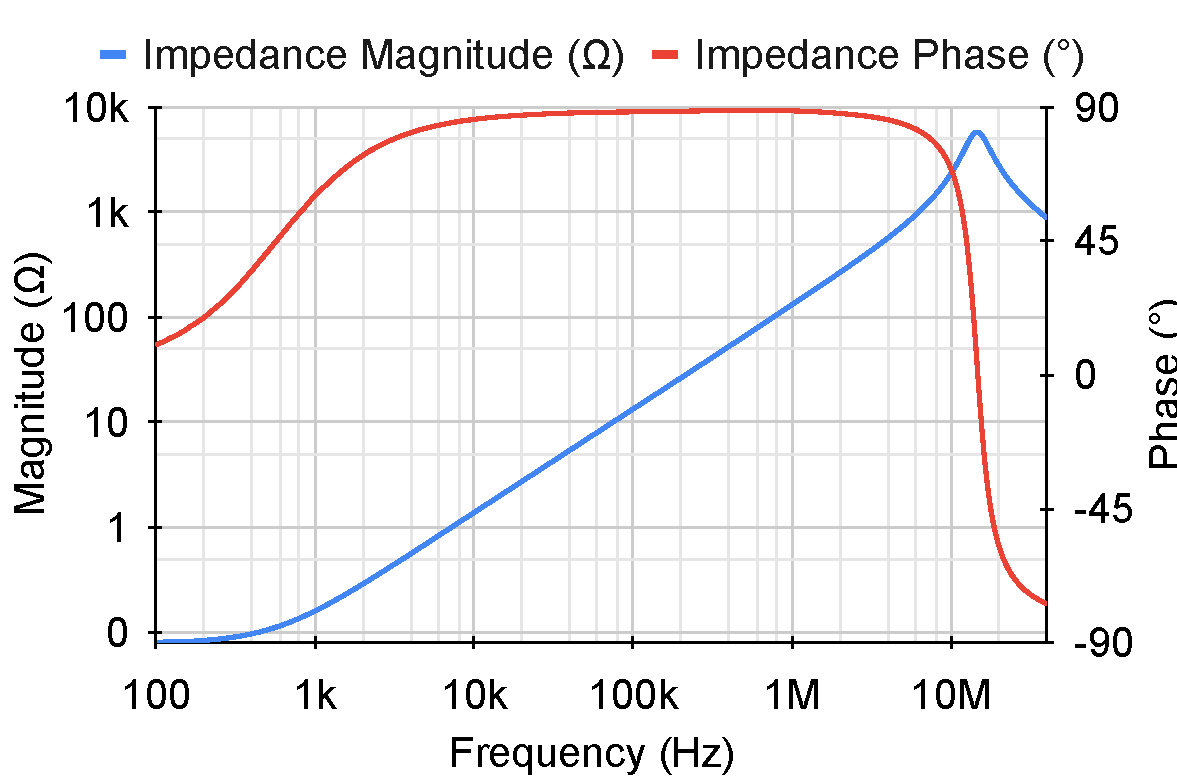
\includegraphics[width=\textwidth]{Bilder/Kapitel3/SER223_BodePlot.pdf}
        \caption{SER1512-223ME complex magnitude and phase vs frequency}
    \end{subfigure}
    \begin{subfigure}[b]{0.50\textwidth}
        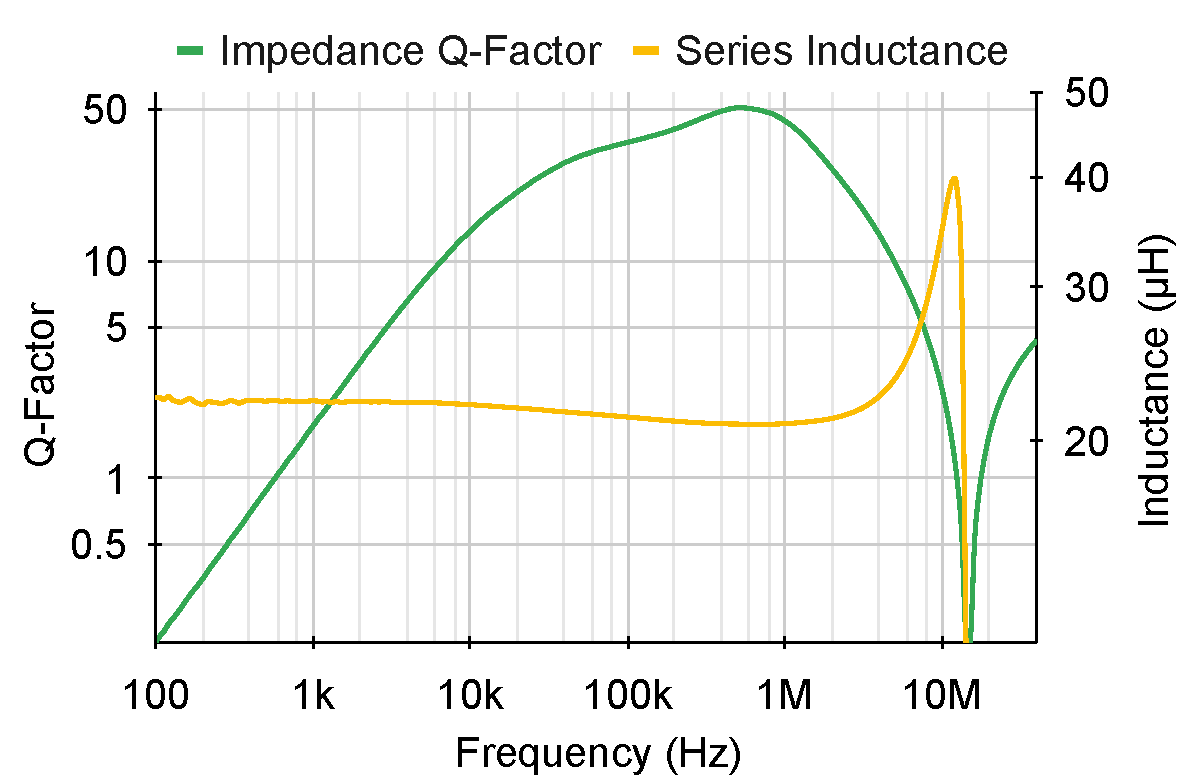
\includegraphics[width=\textwidth]{Bilder/Kapitel3/SER223_QLPlot.pdf}
        \caption{SER1512-223ME \ac{Q-factor} and inductance vs frequency}
    \end{subfigure}
    \caption{Measured frequency response of the SER1512-223ME}
    \label{fig:bode_100_measurements}							
\end{figure}
\section{The Saturation Behaviour of the Inductor} \label{sec:the_saturation_behaviour_of_the_inductor}
To measure the saturation behaviour a "Power Choke Tester" by the manufacturer ed-k was used. It subjects the inductor under test to a rectangular voltage pulse and measures the current through it until a set maximum current is reached. The voltage applied is set to be similar to the actual voltage the inductor is subjected to, here set to \SI{30}{V}. With the voltage and current data, the device is able to calculate the magnetic flux $\Phi$ in the inductor. Calculating the saturation behaviour is done by differentiating the flux.\\ 

The measured saturation behaviours of the \textit{SER1512-223ME}, \textit{UA8014-AL} and \textit{XGL1313-103ME} inductors is displayed in figure \ref{fig:differential_inductance_of_the_ser1512-223me_inductor}. Considering the \textit{SER1512-223ME} inductor, a close to constant inductance with an average of \SI{21.8}{\micro\henry} can be measured up to a current of \SI{5}{\A}, after which the curve decreases following an s-curve. Levelling out at an inductance around \SI{1.18}{\micro\henry}. This means that the inductor enters saturation at around \SI{5}{\A} of \ac{DC} through it, marking this current as the maximum current the inductor should experience without causing the ripple current to increase, resulting in greater power losses.
\begin{figure}[H]
    \centering
    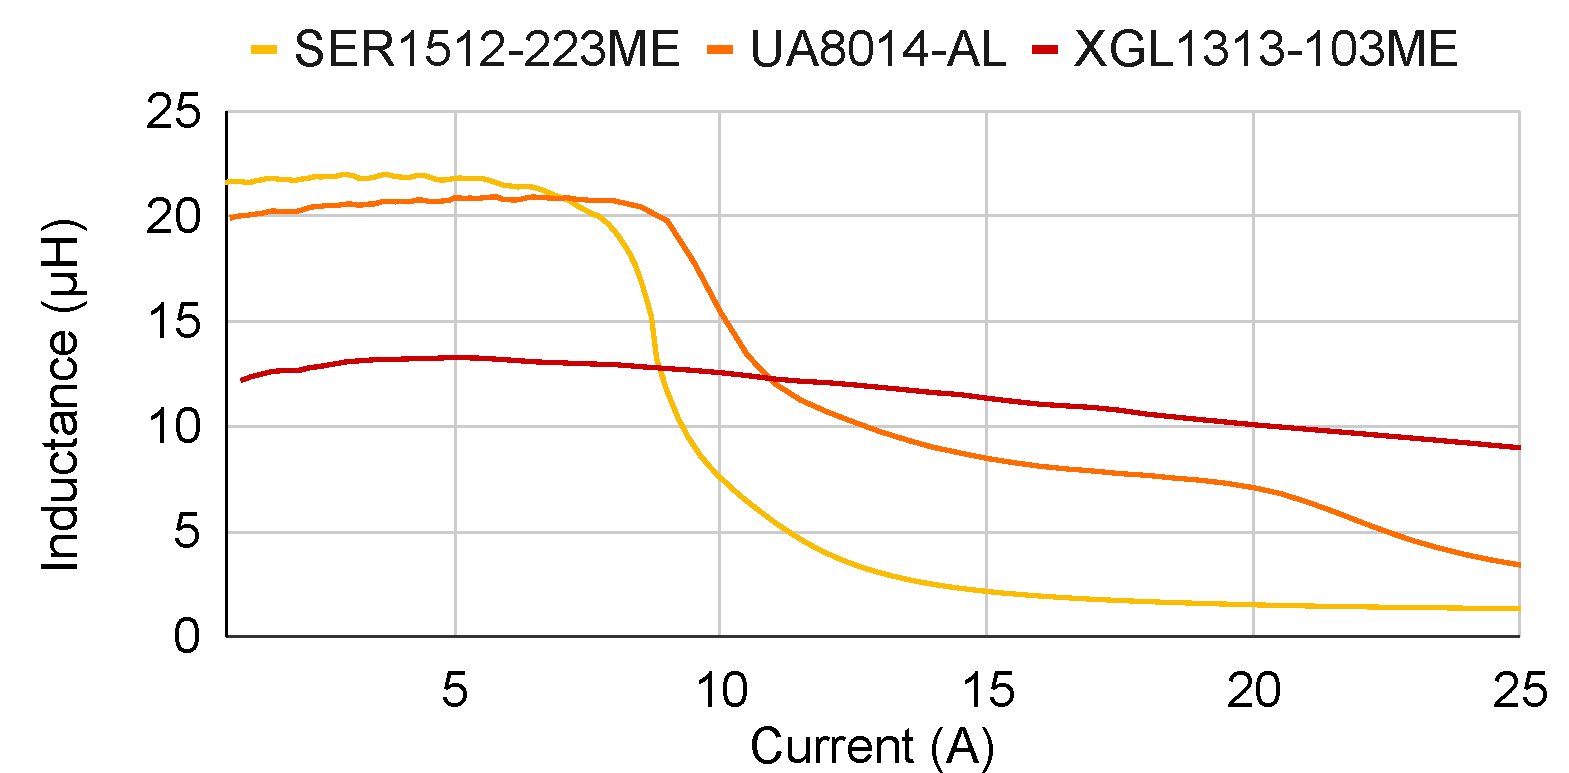
\includegraphics[width=0.8\linewidth]{Bilder//Kapitel3/SER223_UA_XGL103_Saturation.pdf}
    \caption{Differential inductance of the SER1512-223ME and UA8014-AL inductor}
    \label{fig:differential_inductance_of_the_ser1512-223me_inductor}
\end{figure}
The difference in the behaviour of this inductor to the \textit{XGl1313-103ME} inductor can be led back to two reasons. Firstly the \textit{XGL}-inductor is only a \SI{10}{\micro\H} inductor, compared to the \SI{22}{\micro\H} \textit{SER}-inductor, explaining their different initial inductances. Secondly, the very gradual reduction of the saturation of the \textit{XGL}-inductor is a direct consequence of its air gap. As stated in section \ref{sec:the_working_principal_of_the_inductor}, the air gap stretches the saturation graph, leading to a more gradual decline in the inductance and increasing the saturation current.
Being made from composite materials, instead of a ferrite, the \textit{XGL1313-103ME} does not contain a direct gap in the inductor's core. Rather the density of paramagnetic material in the composite powder is charged for different sections of the core material, creating an air gap distributed throughout some parts of the core.

\section{The Hysteresis Behaviour of the Inductor}
In order to measure the hysteresis behaviour of an inductor, the magnetic field $H$ and the magnetic flux density $B$ at any moment in the inductor's charge cycle need to be calculated, as they cannot easily be measured directly. By using Ampere's law of equation \ref{eq:amperes_law} the magnetic field $H$ can be determined by measuring the current through the inductor and 
with the help of the magnetic length $l_m$ and the number of windings $N$.
\begin{equation}\label{eq:amperes_law_toH}
    H = I \cdot \frac{N}{l_m} 
\end{equation}
Similarly, the voltage across the inductor is used to calculate the magnetic flux density $B$, making use of Faraday's law given in equation \ref{eq:faradays_law}. It rearranges to 
\begin{equation}\label{eq:faradays_law_toB}
	B = \frac{1}{N \cdot A_c} \int_0^t v(\tau)d\tau \quad\text{.}   
\end{equation}
Both equations rely on exact measurements of the inductor's magnetic length $l_m$ and crossectional area $A_c$. These measurements are often not provided by the inductor manufacturer, as is the case with all inductors examined in this thesis. To provide a proof of concept of the measurement setup, a custom wound inductor with known core parameters is used. The chosen core from the producer ferroxcube, called PQ20/16 \cite{ferroxcubeMaterialSpecifications3C952015, ferroxcubeProductSpecificationsCore2016}, came with exact values for each of the unknown parameters and a measured hysteresis curve. It provides a direct control to validate the measurement approach while eliminating errors in the measurement of the core's dimensions. The core is wound with 8 windings and pressed together to create an inductor without an air gap. Hereby all variables for the hysteresis measurement are known.
\begin{table}[H]
    \centering
    \caption{Parameters of the custom inductor \cite{ferroxcubeMaterialSpecifications3C952015}}
    \begin{tabular}{|l|c|c|c|c|}
        \hline
        Parameter & Magnetic length $l_m$ &  Air gap length $l_g$ &  Effective area $A_e$ & Windings $N$ \\
        \hline
        Value & \SI{37.8}{\milli\m} & \SI{0}{\milli\m} & \SI{61.9}{\milli\square\m} & 8\\
        \hline
    \end{tabular}
    \label{tab:parameters_of_the_custom_inductor}
\end{table}

Measuring the hysteresis is done by subjecting the inductor under test to a rectangular voltage pulse until the core reaches saturation. After that the voltage is dropped and the inductor discharges on its own. Since there was no dedicated device available, the setup displayed in figure \ref{fig:hysteresis_measurement_setup} needed to be implemented manually.
\begin{figure}[H]
    \centering
    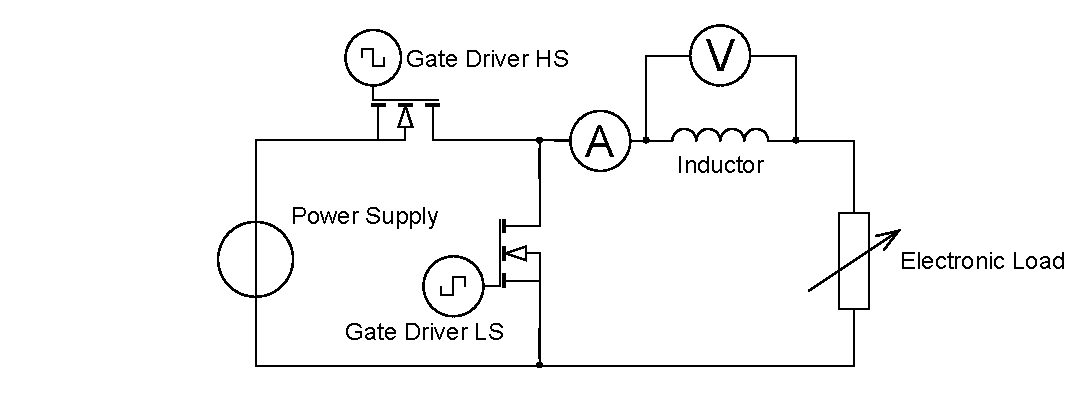
\includegraphics[width=1\linewidth]{Bilder/Kapitel3/Hysteresis_Measurement_Setup.pdf}
    \caption{Hysteresis measurement setup}
    \label{fig:hysteresis_measurement_setup}
\end{figure}
Using a \ac{GaNFET} half-bridge to connect the inductor to and adding a load with capacitive and resistive properties, allows the charging time to be regulated and a reverse current to flow through the inductor. The reverse current is necessary to measure the coercive force $H_c$. Connecting a current clamp to the wire leading to the inductor and a voltage probe across the inductor enables the oscilloscope to measure the hysteresis curve. As the voltage supplied to the inductor determines the rate of change of the inductor current, a lower switching frequency is desirable, as it allows a lower voltage to be used to achieve the same maximum current since more time for the charging process is given.\\
Limiting factors of this setup are the minimum speed the \ac{GaNFET} half-bridge can switch at, the maximum change in current the power supply can deliver and the maximum power spikes the electronic load is able to handle. In this case, the minimum switching speed achieved was \SI{10}{\kilo\Hz}, which is just low enough to enable a clear measurement.\\

Inserting the custom inductor into the measurement setup shown in figure \ref{fig:hysteresis_measurement_setup}, applying a \SI{52}{\V} supply voltage, allowing a maximum \SI{30}{\A} current pull and switching at \SI{13}{\kilo\Hz}, the behaviour shown in image \ref{fig:hysteresis_measurement_of_the_custom_wound_inductor} was created. 
Hysteresis and saturation behaviour are clearly visible. The noise in the measurements at the points where the axes are crossed is not negligible, influencing the values of the remnant B-field $B_r$ and the coercivity $H_c$. Most of this noise is a product of measurement noise, as the oscilloscope needs to measure high voltages and currents, which worsens the resolution at low currents and voltages. The distortion visible at the maximum point of saturation is due to fluctuations in the voltage of the power supply, as it operates at its peak capabilities.
\begin{figure}[H]
    \centering
    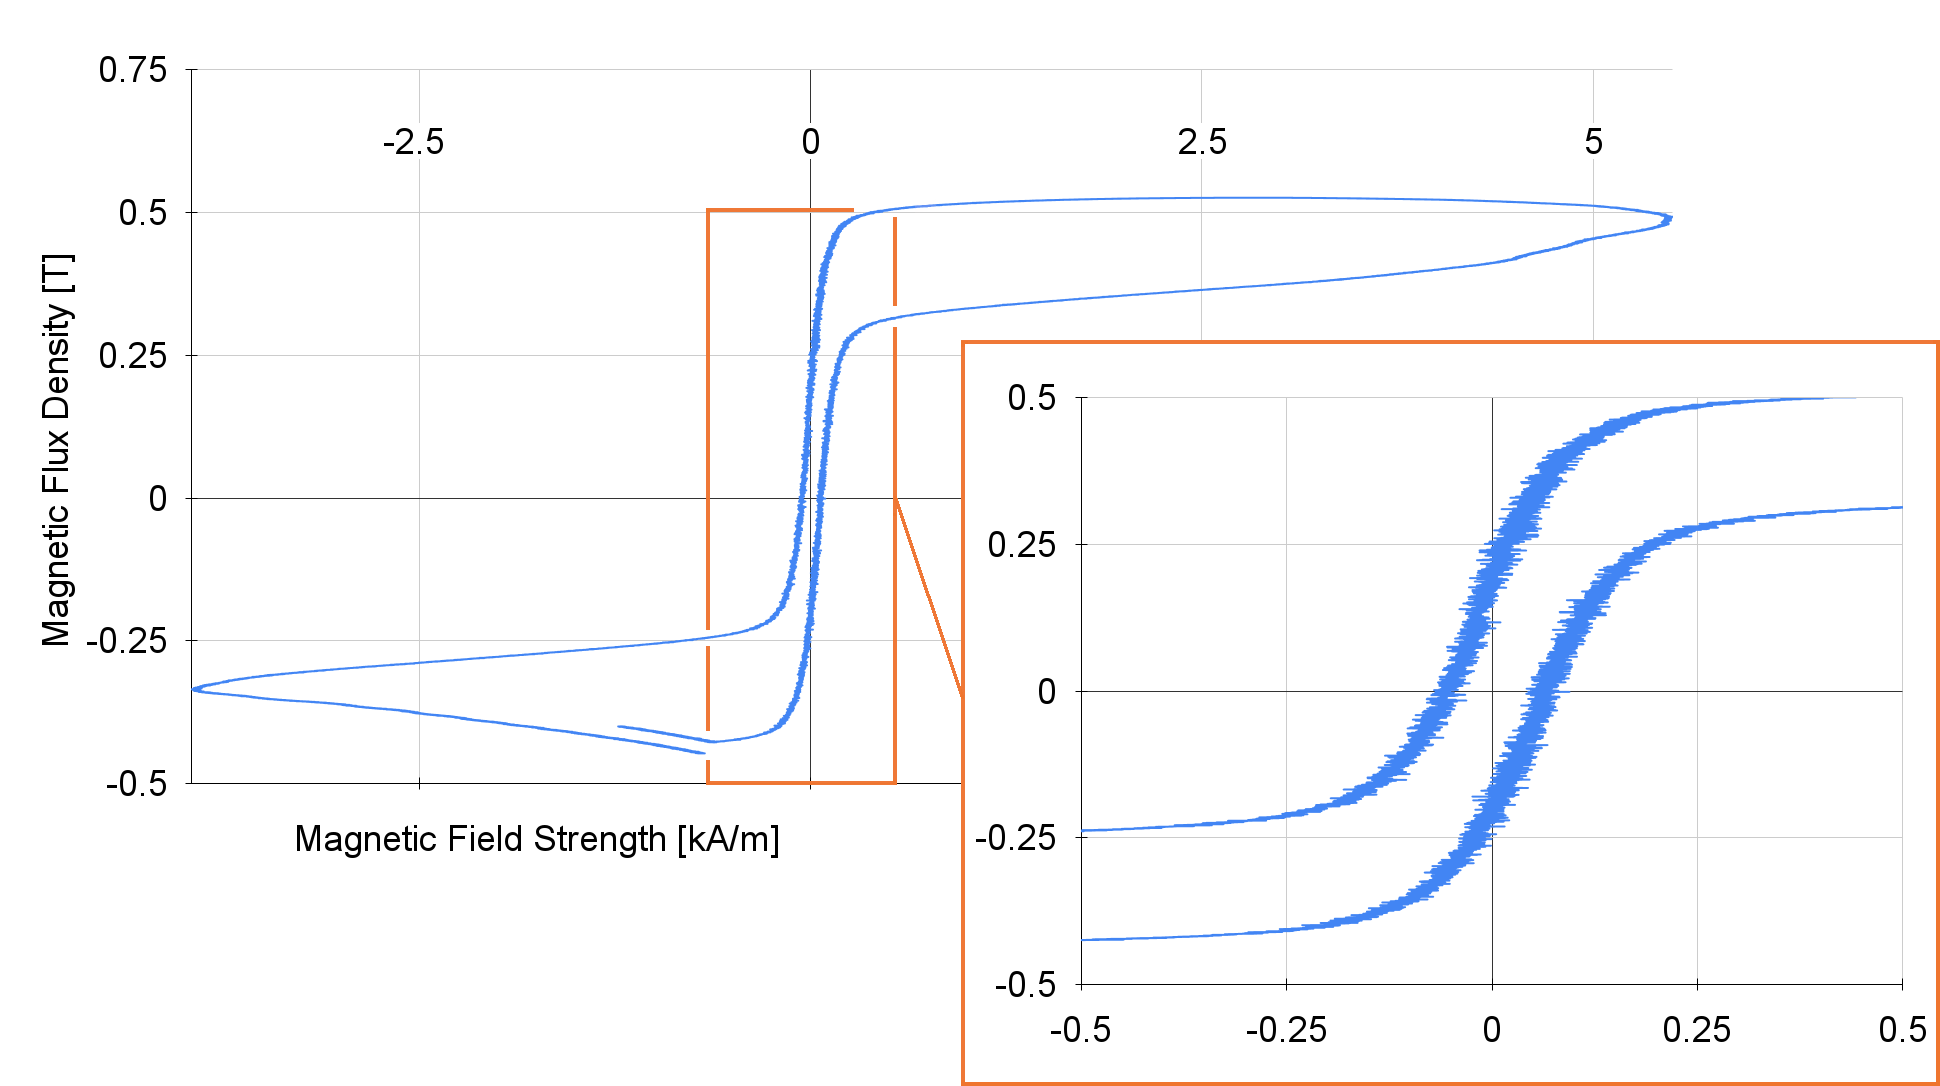
\includegraphics[width=1\linewidth]{Bilder//Kapitel3/Hysteresis_Measurement_3.png}
    \caption{Hysteresis Measurement of the custom wound inductor}
    \label{fig:hysteresis_measurement_of_the_custom_wound_inductor}
\end{figure}
Table \ref{tab:B-H_curve_points_of_interest_comparison} compares the measured points of interest to the data provided by the producer of the core material. While the deviations are noticeable, they are still attributable to the noise and limitations of the setup. If the setup is changed to allow for higher precision at low currents and voltages and the saturation region is not plagued by unwanted behaviour of the power supply and electronic load, the results can be improved. This validates the use of this approach to also measure inductors, whose core parameters are unknown. First, however, the measured results are imported into LTspice to determine the validity of the model in the following chapter.
\begin{table}[H]
    \centering
    \caption{Comparison of B-H curve parameters \cite{ferroxcubeProductSpecificationsCore2016}}
    \begin{tabular}{|l|c|c|}
        \hline
        & Measured & Given by the data sheet \\
        \hline
        Coercive Force $H_c$ & \SI{54}{\A\per\m} & \SI{13}{\A\per\m}\\ 
        \hline
        Remnant B-Field $B_r$ & \SI{255}{\milli\tesla} & \SI{156}{\milli\tesla}\\
        \hline
        Maximum B-Field $B_{max}$ & \SI{570}{\milli\tesla} & \SI{500}{\milli\tesla}\\
        \hline
    \end{tabular}
    \label{tab:B-H_curve_points_of_interest_comparison}
\end{table}



















